\documentclass[11pt,a4paper,final]{article} %draft

\usepackage[T1,T2A]{fontenc}
\usepackage[utf8]{inputenc}
\usepackage[english, russian]{babel}

\usepackage[final]{pdfpages}

\usepackage{textcomp,enumitem}

\usepackage{amsmath,amsthm,amssymb}

\usepackage{fancyhdr} % для настройки страницы и колонтитулов

\usepackage{graphicx}

\usepackage{indentfirst} % автоматический отступ в начале каждого раздела

\usepackage[unicode, pdftex, colorlinks, urlcolor=blue]{hyperref}

\usepackage[left=2cm,right=2cm,top=2cm,bottom=2cm,bindingo ffset=0cm]{geometry}

\linespread{1.3} % устанавливает междустрочный интервал

\pagestyle{plain} % для отображения номеров внизу 

\usepackage{float}

\usepackage{listings} 

\usepackage{pdflscape}
\usepackage{listings} 
\definecolor{darkgreen}{rgb}{0,0.5,0}
\usepackage{subcaption}


\lstset{
	backgroundcolor=\color{white},  % Устанавливаем белый фон для блока кода
	basicstyle=\ttfamily\small\fontfamily{inconsolata}\selectfont,  % Основной стиль текста: моноширинный шрифт Inconsolata с небольшим размером
	commentstyle=\color{darkgreen}\slshape,  % Комментарии будут зелеными и курсивными
	keywordstyle=\color{blue}\bfseries,  % Ключевые слова выделяются синим цветом и полужирным шрифтом
	numberstyle=\scriptsize\color{gray},  % Стиль нумерации строк: маленький размер шрифта и серый цвет
	stringstyle=\color{orange},  % Строки (текст в кавычках) отображаются оранжевым цветом
	breakatwhitespace=false,  % Не прерывать строки только по пробелам
	breaklines=true,  % Автоматический перенос длинных строк
	postbreak=\mbox{\textcolor{gray}{$\hookrightarrow$}}, % Символ переноса строки
	captionpos=b,  % Позиция заголовка/описания для блока кода — внизу (b — bottom)
	keepspaces=true,  % Сохранить пробелы, как они есть, в исходном коде
	numbers=left,  % Нумерация строк будет отображаться слева
	numbersep=5pt,  % Отступ между строками кода и номерами строк (4pt)
	showspaces=false,  % Не показывать пробелы
	showstringspaces=false,  % Не показывать пробелы внутри строк
	showtabs=false,  % Не показывать символы табуляции
	tabsize=4,  % Размер табуляции — 4 пробела
	language=Haskell,  % Указываем язык программирования для синтаксического подсветки (C++)
	captionpos=t,  % Заголовок кода будет размещен вверху (t — top)
	xleftmargin=0mm,  % Убираем отступ слева
	frame=single,  % Однотонная рамка вокруг блока кода
	framerule=0.25mm,  % Толщина рамки — 0.25 мм
	literate=
	{а}{{\selectfont\char224}}1
	{б}{{\selectfont\char225}}1
	{в}{{\selectfont\char226}}1
	{г}{{\selectfont\char227}}1
	{д}{{\selectfont\char228}}1
	{е}{{\selectfont\char229}}1
	{ж}{{\selectfont\char230}}1
	{з}{{\selectfont\char231}}1
	{и}{{\selectfont\char232}}1
	{й}{{\selectfont\char233}}1
	{к}{{\selectfont\char234}}1
	{л}{{\selectfont\char235}}1
	{м}{{\selectfont\char236}}1
	{н}{{\selectfont\char237}}1
	{о}{{\selectfont\char238}}1
	{п}{{\selectfont\char239}}1
	{р}{{\selectfont\char240}}1
	{с}{{\selectfont\char241}}1
	{т}{{\selectfont\char242}}1
	{у}{{\selectfont\char243}}1
	{ф}{{\selectfont\char244}}1
	{х}{{\selectfont\char245}}1
	{ц}{{\selectfont\char246}}1
	{ч}{{\selectfont\char247}}1
	{ш}{{\selectfont\char248}}1
	{щ}{{\selectfont\char249}}1
	{ъ}{{\selectfont\char250}}1
	{ы}{{\selectfont\char251}}1
	{ь}{{\selectfont\char252}}1
	{э}{{\selectfont\char253}}1
	{ю}{{\selectfont\char254}}1
	{я}{{\selectfont\char255}}1
	{А}{{\selectfont\char192}}1
	{Б}{{\selectfont\char193}}1
	{В}{{\selectfont\char194}}1
	{Г}{{\selectfont\char195}}1
	{Д}{{\selectfont\char196}}1
	{Е}{{\selectfont\char197}}1
	{Ж}{{\selectfont\char198}}1
	{З}{{\selectfont\char199}}1
	{И}{{\selectfont\char200}}1
	{Й}{{\selectfont\char201}}1
	{К}{{\selectfont\char202}}1
	{Л}{{\selectfont\char203}}1
	{М}{{\selectfont\char204}}1
	{Н}{{\selectfont\char205}}1
	{О}{{\selectfont\char206}}1
	{П}{{\selectfont\char207}}1
	{Р}{{\selectfont\char208}}1
	{С}{{\selectfont\char209}}1
	{Т}{{\selectfont\char210}}1
	{У}{{\selectfont\char211}}1
	{Ф}{{\selectfont\char212}}1
	{Х}{{\selectfont\char213}}1
	{Ц}{{\selectfont\char214}}1
	{Ч}{{\selectfont\char215}}1
	{Ш}{{\selectfont\char216}}1
	{Щ}{{\selectfont\char217}}1
	{Ъ}{{\selectfont\char218}}1
	{Ы}{{\selectfont\char219}}1
	{Ь}{{\selectfont\char220}}1
	{Э}{{\selectfont\char221}}1
	{Ю}{{\selectfont\char222}}1
	{Я}{{\selectfont\char223}}1,
	numbers=left, % пронумеровать строки с левой стороны
	breaklines=true % разрешает автоматический перенос строк
}

\hypersetup{
	colorlinks=true, % делает ссылки цветными вместо рамки
	linkcolor=blue, % цвет внутренних ссылок
	urlcolor=blue, % цвет внешних ссылок
	citecolor=blue % цвет ссылок на литературу в тексте
}

\textheight=24cm 
\textwidth=16cm
\oddsidemargin=0pt 
\topmargin=-1.5cm
\parindent=24pt 
\parskip=0pt 
\tolerance=2000 
\flushbottom 

%\usepackage[font=scriptsize]{caption}
\usepackage[labelsep=period]{caption}

\usepackage{amsmath}
\usepackage{multirow} 
\usepackage{tabularx}
\usepackage{subfig}

\newcommand{\specialcell}[2][l]{\begin{tabular}[#1]{@{}l@{}}#2\end{tabular}}

\begin{document}
	
	\thispagestyle{empty}
	
	\begin{center}
		{\Large МИНОБРНАУКИ РОССИИ}\\
		~\\
		{\large ФЕДЕРАЛЬНОЕ ГОСУДАРСТВЕННОЕ БЮДЖЕТНОЕ ОБРАЗОВАТЕЛЬНОЕ УЧРЕЖДЕНИЕ ВЫСШЕГО ПРОФЕССИОНАЛЬНОГО ОБРАЗОВАНИЯ}\\
		~\\
		{\Large \bf <<САНКТ-ПЕТЕРБУРГСКИЙ ПОЛИТЕХНИЧЕСКИЙ УНИВЕРСИТЕТ ПЕТРА ВЕЛИКОГО>>}\\
		~\\
		{\large Институт компьютерных наук и кибербезопасности }\\
		{\large Высшая школа технологий искусственного интеллекта}\\
		{\large Направление 02.03.01 Математика и компьютерные науки}\\
		~\\
		~\\
		~\\
		~\\
		{\Large \bf  Отчет по лабораторной работе №3 }\\
		\vspace{3mm}
		{\Large {по дисциплине <<Функциональное программирование>>}}\\
		\vspace{3mm}
		{\Large {Вариант 4}}\\
		~\\
		~\\
		~\\
		~\\
		~\\
		~\\
		{\large Обучающийся: \underline{\hspace{3.5cm}} \hspace{12mm} Шихалев А.О.}\\
		~\\
		{\large Руководитель: \underline{\hspace{3.5cm}} \hspace{12mm} Моторин Д.Е.}\\
		~\\
		~\\
		~\\
		~\\
		~\\
	\end{center}
	\begin{flushright}
		
		«\underline{\hspace{1cm}}»\underline{\hspace{3cm}}20\underline{\hspace{0.7cm}}г.
	\end{flushright}
	~\\
	~\\
	\begin{center}
		{\large Санкт-Петербург, 2024}
	\end{center}
	
\newpage

\tableofcontents

\newpage
\section*{Введение}
\addcontentsline{toc}{section}{Введение}
Практическое задание №3 представляет собой реализацию следующего задания: 

\begin{enumerate}
	\item Найти портрет указанного человека:
	\begin{center}
		\textbf{Ковалевская, Софья Васильевна}
	\end{center}
	\item Перевести изображение в формат .bmp (24-разрядный), при необходимости изменить ширину и высоту изображения без искажений. Сохранить в файл формата .txt фрагмент биографии (не менее 1000 символов без пробелов, текст не должен обрываться на середине слова или предложения). Закодировать текст в изображение методом: 

	\begin{center}
		\textbf{Шифром Цезаря. Смещение задается пользователем}
	\end{center}
	Ключ к шифру записывается в имя файла. Написать функцию расшифровывающую текст из изображения используя ключ из имени файла и сохраняющую результат в отдельный текстовый файл.
	
	\item Создать функции, шифрующие текст последний бит каждого байта, последние два бита каждого байта, ..., все биты в байте. В отчете привести примеры искажений изображения.
	
	\item Написать второй вариант функции, шифрующую текст в изображение, а именно закодировать битовую последовательность зашифрованного текста следующим образом: 
	\begin{itemize}
		\item все чётные биты -- в канал RED;
		\item все нечётные биты -- в канал GREEN;
		\item исходную битовую последовательность канала BLUE инвертировать.
	\end{itemize}
\end{enumerate}

\par Лабораторная работа выполнена на языке Haskell в текстовом редакторе Visual Studio Code 1.95.3.

\newpage
\section {Математическое описание}
\subsection{Шифр Цезаря}
Шифр Цезаря (лат. Notae Caesarianae), также известный как шифр сдвига или код Цезаря — разновидность шифра подстановки, в котором каждый символ в открытом тексте заменяется символом, находящимся на некотором постоянном числе позиций левее или правее него в алфавите (так, в шифре со сдвигом вправо на 3, А была бы заменена на Г, Б станет Д, и так далее). Шифр был назван в честь римского полководца Гая Юлия Цезаря, использовавшего его для секретной переписки со своими военачальниками.

Если сопоставить каждому символу алфавита его порядковый номер (нумеруя с 0), то шифрование и дешифрование можно выразить формулами модульной арифметики~\cite{caesar}:
\[
y = (x + k) \mod n
\]
\[
x = (y - k) \mod n
\]
где: \\
$x$ — символ открытого текста, \\
$y$ — символ шифрованного текста, \\
$n$ — мощность алфавита, \\
$k$ — ключ.


\newpage
\section {Особенности реализации}
\subsection{Исходное изображение и текст}
Для выполнения лабораторной работы необходимо было найти изображение Ковалевской Софьи Васильевны (\hyperref[fig:sonya]{см. рис.~\ref{fig:sonya}}). Изображение было переведено из формата \texttt{jpeg} в формат \texttt{bmp} с помощью сайта~\cite{convertio}.

\begin{figure}[H]
	\centering
	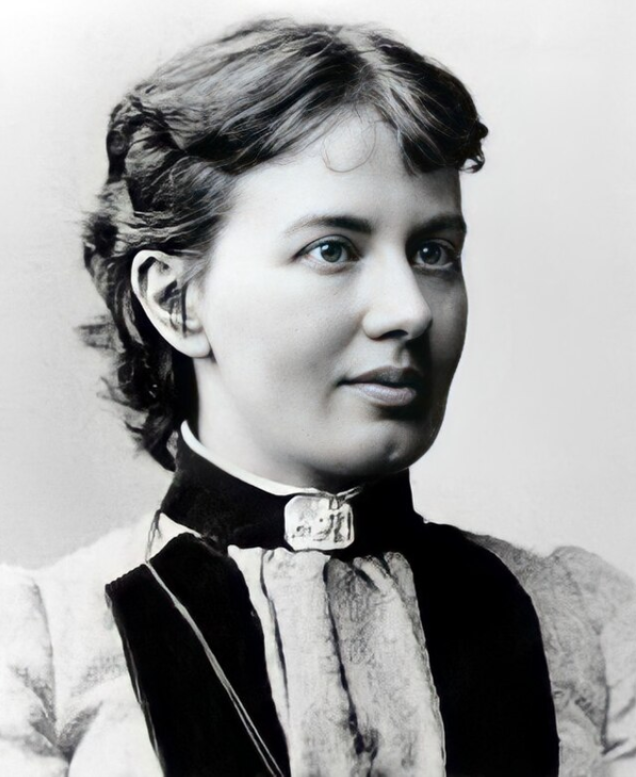
\includegraphics[width=0.6 \linewidth]{img/sonya.png}
	\caption{Изображение Ковалевской С.В.}
	\label{fig:sonya}
\end{figure}


Отрывок биографии Ковалевской Софьи Васильевны длиною в 1442 символа без учёта пробелов представлен ниже.

\lstinline[stringstyle=\color{black}, keywordstyle=\color{black}\bfseries]|Sofya Vasilyevna Kovalevskaya (born January 15, 1850, Moscow, Russia, died February 10, 1891, Stockholm, Sweden) was a mathematician and writer who made a valuable contribution to the theory of partial differential equations. She was the first woman in modern Europe to gain a doctorate in mathematics, the first to join the editorial board of a scientific journal, and the first to be appointed professor of mathematics. In 1868 Kovalevskaya entered into a marriage of convenience with a young paleontologist, Vladimir Kovalevsky, in order to leave Russia and continue her studies. The pair traveled together to Austria and then to Germany, where in 1869 she studied at the University of Heidelberg under the mathematicians Leo Konigsberger and Paul du Bois-Reymond and the physicist Hermann von Helmholtz. The following year she moved to Berlin, where, having been refused admission to the university on account of her gender, she studied privately with the mathematician Karl Weierstrass. In 1874 she presented three papers on partial differential equations, on Saturn's rings, and on elliptic integrals to the University of Gottingen as her doctoral dissertation and was awarded the degree summa cum laude in absentia. Her paper on partial differential equations, the most important of the three papers, won her valuable recognition within the European mathematical community. It contains what is now commonly known as the Cauchy-Kovalevskaya theorem, which gives conditions for the existence of solutions to a certain class of partial differential equations. Having gained her degree, she returned to Russia, where her daughter was born in 1878. She separated permanently from her husband in 1881.|

\subsection{Кодирование и декодирование текста с помощью шифра Цезаря}

Код функций для кодирования и декодирования текста с помощью шифра Цезаря представлен в листинге \hyperref[lst:l1]{листинге 1}. Функция \texttt{encryptCaesar} принимает алфавит в виде списка символов, смещение и сам текст, а возвращает зашифрованный текст. В её коде используется вспомогательная функция \texttt{indexOfSymbol}. Функция принимает список и элемент списка, а возвращает индекс этого элемента. Для создания алфавита используется функция \texttt{createAlphabetFromText}. Она принимает текст, а возвращает алфавит, который в нём используется, в виде списка символов. Для декодирования текста используется функция \texttt{decryptCaesar}, которая, по-сути, является лишь обёрткой над функцией \texttt{encryptCaesar}, так как процесс кодирования осуществляется почти так же как и декодирования. Функция \texttt{decryptCaesar} принимает на вход алфавит, смещение и закодированный текст, а возвращает декодированный текст.

\begin{lstlisting}[caption={Функции для кодирования и декодирования текста с помощью шифра Цезаря.}, label={lst:l1}]
	
createSpecialChars :: [Char]
createSpecialChars = [' ', '!', '(', ')', ',', '-','.', ':', ';', '?', '\'']

createAlphabet :: [Char]
createAlphabet = ['A'..'Z'] ++ ['a'..'z'] ++ ['0'..'9'] ++ createSpecialChars

encryptCaesar :: [Char] -> Int -> String -> String
encryptCaesar alphabet shift text = map caesarChar text
where
caesarChar c = alphabet !! ((indexOf alphabet c + shift) `mod` length alphabet)        

indexOfSymbol :: [Char] -> Char -> Int
indexOfSymbol alphabet symbol = 
case elemIndex symbol alphabet of
Just idx -> idx
Nothing -> error "Character not found in alphabet!!!"


encryptCaesar :: [Char] -> Int -> String -> String
encryptCaesar alphabet shiftCaesar text = map caesarChar text
where 
caesarChar c = alphabet !! ((indexOfSymbol alphabet c + shiftCaesar) `mod` length alphabet)

decryptCaesar :: [Char] -> Int -> String -> String
decryptCaesar alphabet shift = 
encryptCaesar alphabet (alphabetLength - (shift `mod` alphabetLength)) 
where
alphabetLength = length alphabet
\end{lstlisting}

Пример закодированного с помощью шифра Цезаря текста биографии Ковалевской Софьи Васильевны для смещения 5 представлен ниже.

\lstinline[stringstyle=\color{black}]|Xtk3f,afxnq3j0sf,Pt0fqj0xpf3f,:gtws,Ofszfw3,6 ?,6( 5?,Rtxht1?,Wzxxnf?,inji,Kjgwzfw3,65?,6()6?,Xythpmtqr?,X1jijs;,1fx,f,rfymjrfynhnfs,fsi,1wnyjw,1mt,rfij,f,0fqzfgqj,htsywngzynts,yt,ymj,ymjtw3,tk,ufwynfq,inkkjwjsynfq,jvzfyntsxA,Xmj,1fx,ymj,knwxy,1trfs,ns,rtijws,Jzwtuj,yt,lfns,f,ithytwfyj,ns,rfymjrfynhx?,ymj,knwxy,yt,otns,ymj,jinytwnfq,gtfwi,tk,f,xhnjsynknh,otzwsfq?,fsi,ymj,knwxy,yt,gj,fuutnsyji,uwtkjxxtw,tk,rfymjrfynhxA,Ns,6(!(,Pt0fqj0xpf3f,jsyjwji,nsyt,f,rfwwnflj,tk,hts0jsnjshj,1nym,f,3tzsl,ufqjtsytqtlnxy?,aqfinrnw,Pt0fqj0xp3?,ns,twijw,yt,qjf0j,Wzxxnf,fsi,htsynszj,mjw,xyzinjxA,Ymj,ufnw,ywf0jqji,ytljymjw,yt,Fzxywnf,fsi,ymjs,yt,Ljwrfs3?,1mjwj,ns,6(!),xmj,xyzinji,fy,ymj,Zsn0jwxny3,tk,Mjnijqgjwl,zsijw,ymj,rfymjrfynhnfsx,Qjt,Ptsnlxgjwljw,fsi,Ufzq,iz,Gtnx'Wj3rtsi,fsi,ymj,um3xnhnxy,Mjwrfss,0ts,Mjqrmtqy4A,Ymj,ktqqt1nsl,3jfw,xmj,rt0ji,yt,Gjwqns?,1mjwj?,mf0nsl,gjjs,wjkzxji,firnxxnts,yt,ymj,zsn0jwxny3,ts,fhhtzsy,tk,mjw,ljsijw?,xmj,xyzinji,uwn0fyjq3,1nym,ymj,rfymjrfynhnfs,Pfwq,bjnjwxywfxxA,Ns,6("9,xmj,uwjxjsyji,ymwjj,ufujwx,ts,ufwynfq,inkkjwjsynfq,jvzfyntsx?,ts,XfyzwsEx,wnslx?,fsi,ts,jqqnuynh,nsyjlwfqx,yt,ymj,Zsn0jwxny3,tk,Ltyynsljs,fx,mjw,ithytwfq,inxxjwyfynts,fsi,1fx,f1fwiji,ymj,ijlwjj,xzrrf,hzr,qfzij,ns,fgxjsynfA,Mjw,ufujw,ts,ufwynfq,inkkjwjsynfq,jvzfyntsx?,ymj,rtxy,nrutwyfsy,tk,ymj,ymwjj,ufujwx?,1ts,mjw,0fqzfgqj,wjhtlsnynts,1nymns,ymj,Jzwtujfs,rfymjrfynhfq,htrrzsny3A,Ny,htsyfnsx,1mfy,nx,st1,htrrtsq3,pst1s,fx,ymj,Hfzhm3'Pt0fqj0xpf3f,ymjtwjr?,1mnhm,ln0jx,htsinyntsx,ktw,ymj,j2nxyjshj,tk,xtqzyntsx,yt,f,hjwyfns,hqfxx,tk,ufwynfq,inkkjwjsynfq,jvzfyntsxA,Mf0nsl,lfnsji,mjw,ijlwjj?,xmj,wjyzwsji,yt,Wzxxnf?,1mjwj,mjw,ifzlmyjw,1fx,gtws,ns,6("(A,Xmj,xjufwfyji,ujwrfsjsyq3,kwtr,mjw,mzxgfsi,ns,6((6A|


\subsection{Представление текста в виде последовательности бит}

Код функций для преобразования текста в последовательность бит и обратно представлен в листинге~\ref{lst:bit}. Функция \texttt{textToBits} принимает текст в виде строки и возвращает его представление в виде вектора бит. Она использует вспомогательную функцию \texttt{charToBits}, которая преобразует символ в список бит, представляющих его код ASCII в двоичном виде. Для преобразования последовательности бит обратно в текст используется функция \texttt{bitsToText}. Она рекурсивно делит вектор бит на блоки по 8 бит, преобразует каждый блок в символ ASCII и объединяет их в строку. В процессе этого преобразования используется функция \texttt{bitsToInt}, которая преобразует вектор бит в целое число, интерпретируя их как двоичное представление этого числа.


\begin{lstlisting}[caption={Функции для конвертации текста в последовательность бит и обратно.}, label={lst:bit}]
textToBits :: String -> VU.Vector Int
textToBits text = VU.fromList $ concatMap charToBits text

charToBits :: Char -> [Int]
charToBits c = [if testBit (ord c) i then 1 else 0 | i <- [7,6..0]]

bitsToText :: VU.Vector Int -> String
bitsToText bits
| VU.null bits = []
| otherwise = (chr $ bitsToInt (VU.take 8 bits)) : bitsToText (VU.drop 8 bits)

bitsToInt :: VU.Vector Int -> Int
bitsToInt bits = 
sum [bit * (2 ^ index) | (bit, index) <- zip (VU.toList bits) [len,(len - 1)..0]]
where
len = VU.length bits - 1
\end{lstlisting}


\subsection{Работа с файлами}
Для работы с текстовыми файлами использовались базовые функции Haskell -- \texttt{readFile} (читает содержимое файла и возвращает его как строку) и \texttt{writeFile} (записывает строку в файл, заменяя его содержимое).

Для работы с изображениями использовалась библиотека \texttt{JuicyPixels}~\cite{JuicyPixels}. С её помощью можно как прочитать изображение в любом популярном формате, так и сохранить его. В частности в работе использовались функции: \texttt{readImage} -- для чтения изображения из указанного файла, \texttt{saveBmpImage} -- для сохранения изображения в формате bmp.


\subsection{Сохранение зашифрованных данных в изображении}
\subsubsection{Первый вариант функции}

Код функций для создания изображения с закодированными данными представлен в листинге~\ref{lst:genImg}. Функция \texttt{encodePixel} отвечает за кодирование последовательности бит в определённый пиксель изображения. Она принимает количество бит данных, которое будет сохранено в каждый байт изображения, исходное изображение, вектор бит зашифрованных данных, координаты пикселя (\(x, y\)) и возвращает новый пиксель с закодированными данными. Для этого функция вычисляет индекс пикселя в изображении, извлекает соответствующую часть вектора бит данных, преобразует её в целые числа, накладывает битовую маску, которая соответствует количество изменяемых бит в байте, и записывает закодированные данные. Для создания маски используется вспомогательная функция \texttt{createMask}.

Функция \texttt{encodePixel} затем используется вместе с функцией \texttt{generateImage} из библиотеки JuicyPixels для генерации нового изображения.

При сохранении изображения в файл, в его названии сохраняется смещение шифра Цезаря и количество бит в байте, отведённых для хранения зашифрованных данных. Например, название изображения \texttt{sofya\_2\_10.bmp} означает, что при кодировании использовался код Цезаря со смещением 10, а для хранения закодированных данных в каждом байте изображения использовалось 2 бита.

\begin{lstlisting}[caption={Функции для создания изображения с закодированными данными.}, label={lst:genImg}]
createMask :: Int -> Int
createMask shift = shiftL (complement 0) shift .&. complement 0

encodePixel :: Int -> Image PixelRGB8 -> VU.Vector Int -> Int -> Int -> PixelRGB8
encodePixel bitsPerByte img bits x y = PixelRGB8 newR newG newB
where
width = imageWidth img

index = x + y * width
startPos = index * 3 * bitsPerByte
pixelBits = VU.slice startPos (3 * bitsPerByte) bits

bitsIntR = bitsToInt $ VU.slice 0 bitsPerByte pixelBits
bitsIntG = bitsToInt $ VU.slice bitsPerByte bitsPerByte pixelBits
bitsIntB = bitsToInt $ VU.slice (2 * bitsPerByte) bitsPerByte pixelBits

mask = createMask bitsPerByte

PixelRGB8 r g b = pixelAt img x y
newR = intToWord8 $ ((word8ToInt r) .&. mask) .|. bitsIntR
newG = intToWord8 $ ((word8ToInt g) .&. mask) .|. bitsIntG
newB = intToWord8 $ ((word8ToInt b) .&. mask) .|. bitsIntB
\end{lstlisting}


\subsubsection{Второй вариант функции}

Второй вариант функции \texttt{encodePixel} аналогичен первому, но с некоторыми изменениями в логике извлечения бит и обработки пикселей. Эта функция принимает такие же параметры, как и в первом варианте: количество бит данных, которые будут сохранены в каждый байт изображения, исходное изображение, вектор бит зашифрованных данных, координаты пикселя (\(x, y\)) и возвращает новый пиксель с закодированными данными.

Особенностью второго варианта является использование функции \texttt{VectorU.ifilter}, которая позволяет извлекать биты для каждого канала (красного и зелёного) по отдельности. Для канала красного (\texttt{R}) извлекаются биты с чётными индексами, а для зелёного (\texttt{G}) — с нечётными индексами. Это достигается с помощью фильтрации индексов, где для каждого индекса проверяется, является ли он чётным или нечётным. Кроме того, для синего канала (\texttt{B}) применяется операция дополнения (комплемента) значения цвета.

После извлечения битов для каждого канала они преобразуются в целые числа с помощью функции \texttt{bitsToInt}, и затем эти значения накладываются на исходные значения пикселя с использованием битовой маски, создаваемой функцией \texttt{createMask}.

Функция \texttt{encodePixel} затем используется в сочетании с функцией \texttt{generateImage} из библиотеки JuicyPixels для генерации нового изображения.

\begin{lstlisting}[caption={Второй вариант функции сохранения зашифрованных данных в изображение}, label={lst:genImg2}]
encodePixel :: Int -> Image PixelRGB8 -> VectorU.Vector Int -> Int -> Int -> PixelRGB8
encodePixel bitsPerByte img bits x y = PixelRGB8 newR newG newB
where
width = imageWidth img

index = x + y * width
startPos = index * 2 * bitsPerByte
pixelBits = VectorU.slice startPos (2 * bitsPerByte) bits

bitsIntR = bitsToInt $ VectorU.ifilter (\i _ -> i `mod` 2 == 0) pixelBits
bitsIntG = bitsToInt $ VectorU.ifilter (\i _ -> i `mod` 2 == 1) pixelBits

mask = createMask bitsPerByte

PixelRGB8 r g b = pixelAt img x y
newR = intToWord8 $ ((word8ToInt r) .&. mask) .|. bitsIntR
newG = intToWord8 $ ((word8ToInt g) .&. mask) .|. bitsIntG
newB = complement b
\end{lstlisting}


\subsection{Чтение зашифрованных данных из изображения}

\subsubsection{Первый вариант}

Код функций для чтения зашифрованных данных из изображения представлен в листинге~\ref{lst:readImg}. Функция \texttt{extractBits} извлекает заданное количество бит из одного байта пикселя. Она принимает число бит на байт и байт пикселя, возвращая список бит. Функция \texttt{extractBitsFromPixel} предназначена для извлечения бит из всех трёх цветовых каналов (\(R, G, B\)) пикселя. Она объединяет списки бит из каждого канала в один общий список. Для извлечения бит из всего изображения используется функция \texttt{extractBitsFromImage}. Она последовательно обрабатывает все пиксели изображения, извлекая биты с помощью \texttt{extractBitsFromPixel}, и объединяет их в общий список.

Функция \texttt{extractShift} извлекает смещения для шифра Цезаря из названия файла изображения.

\begin{lstlisting}[caption={Функции для чтения зашифрованных данных из изображения.}, label={lst:readImg}]
extractBits :: Int -> Pixel8 -> [Int]
extractBits bitsPerByte pixelByte = 
[ if testBit pixelByte i then 1 else 0 | i <- [bitsPerByte-1, bitsPerByte-2..0] ] 

extractBitsFromPixel :: Int -> PixelRGB8 -> [Int]
extractBitsFromPixel bitsPerByte (PixelRGB8 r g b) =
let bitsR = extractBits bitsPerByte r
	bitsG = extractBits bitsPerByte g
	bitsB = extractBits bitsPerByte b
in bitsR ++ bitsG ++ bitsB

extractBitsFromImage :: Int -> Image PixelRGB8 -> [Int]
extractBitsFromImage bitsPerByte img = 
let width = imageWidth img
	height = imageHeight img
	pixels = [ pixelAt img x y | y <- [0..height - 1], x <- [0..width - 1] ]
in concatMap (extractBitsFromPixel bitsPerByte) pixels

extractShift :: String -> Maybe Int
extractShift path = 
let shift = takeWhile (`elem` ['0'..'9']) (reverse $ takeWhile (/= '_') (reverse path))
in readMaybe shift
\end{lstlisting}

\subsubsection{Второй вариант}

 Основное отличие второго варианта заключается в способе обработки бит из цветовых каналов. В данном подходе функция \texttt{extractBitsFromPixel} чередует биты из красного (\(R\)) и зелёного (\(G\)) каналов, создавая общий список бит в порядке их чередования. Для реализации этого используется вспомогательная функция \texttt{interleave}, которая принимает два списка и чередует их элементы.

Функция \texttt{extractBitsFromPixel} принимает количество бит на байт и пиксель (\texttt{PixelRGB8}), извлекая биты из каналов \(R\) и \(G\) с использованием функции \texttt{extractBits}. Затем с помощью функции \texttt{interleave} списки бит из каналов \(R\) и \(G\) объединяются в один список с чередованием элементов. 

Функции \texttt{extractBits} и \texttt{extractBitsFromImage} остаются такими же, как в первом варианте, но теперь используют модифицированную \texttt{extractBitsFromPixel}. Использование функции \texttt{interleave} позволяет упорядочить биты из двух списков в чередующемся порядке. Второй вариант функции texttt{extractBitsFromPixel} извлечение битов из пикселей изображения представлен в листинге~\ref{lst:readImg2}.

\begin{lstlisting}[caption={Функции для чтения зашифрованных данных из изображения (второй вариант).}, label={lst:readImg2}]

extractBitsFromPixel :: Int -> PixelRGB8 -> [Int]
extractBitsFromPixel bitsPerByte (PixelRGB8 r g b) =
let bitsR = extractBits bitsPerByte r
    bitsG = extractBits bitsPerByte g
    interleave [] [] = []
    interleave (x:xs) [] = x : interleave xs []
    interleave [] (y:ys) = y : interleave [] ys
    interleave (x:xs) (y:ys) = x : y : interleave xs ys
in interleave bitsR bitsG
\end{lstlisting}




 \newpage
\section {Результаты работы программы}
\subsection{Первый вариант}
При успешном завершении программа создаёт три файла: файл изображения с закодированных текстом, текстовый файл с закодированным текстом и текстовый файл с декодированным текстом.

\begin{figure}[h]
	\centering
	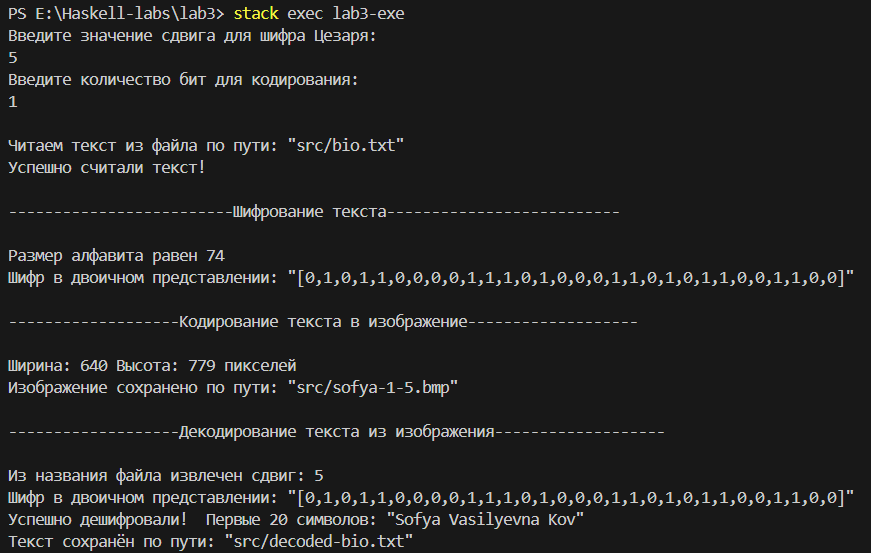
\includegraphics[width=0.85\linewidth]{img/results.png}
	\caption{Результаты работы программы в консоли.}
	\label{fig:results}
\end{figure}

На Рис.~\ref{fig:results} представлены результаты работы программы в консоли.

% Первая строка на первой странице
\begin{figure}[h!]
	\centering
	\begin{subfigure}[b]{0.3\linewidth}
		\centering
		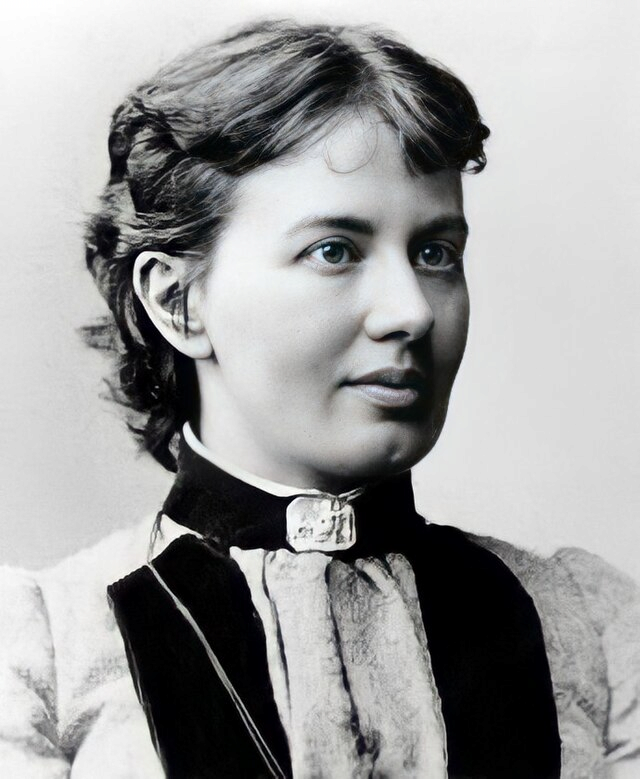
\includegraphics[width=\linewidth]{img/sofya-1-5.png}
		\caption{1 бит.}
		\label{fig:p1}
	\end{subfigure}
	\hfill
	\begin{subfigure}[b]{0.3\linewidth}
		\centering
		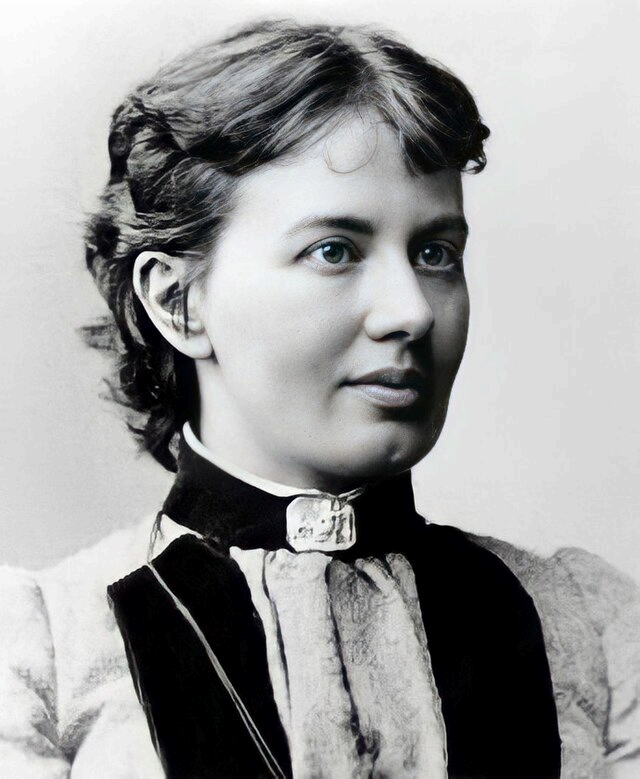
\includegraphics[width=\linewidth]{img/sofya-2-5.png}
		\caption{2 бита.}
		\label{fig:p2}
	\end{subfigure}
	\hfill
	\begin{subfigure}[b]{0.3\linewidth}
		\centering
		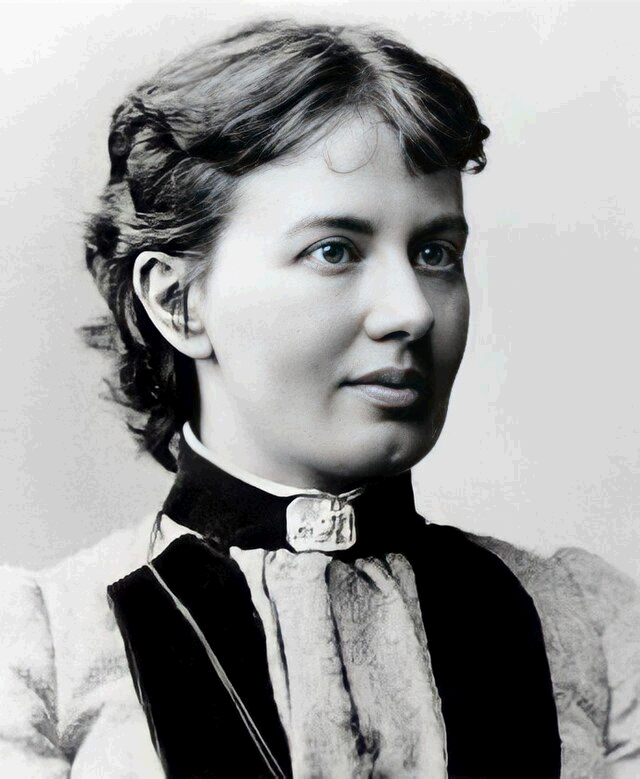
\includegraphics[width=\linewidth]{img/sofya-3-5.png}
		\caption{3 бита.}
		\label{fig:p3}
	\end{subfigure}
	
	\caption{Изображения с зашифрованными данными.}
	\label{fig:encrypted_images_row1}
\end{figure}

% Вторая часть: нумерация с d
\begin{figure}[h!]
	\centering
	
	\begin{subfigure}[b]{0.3\linewidth}
		\centering
		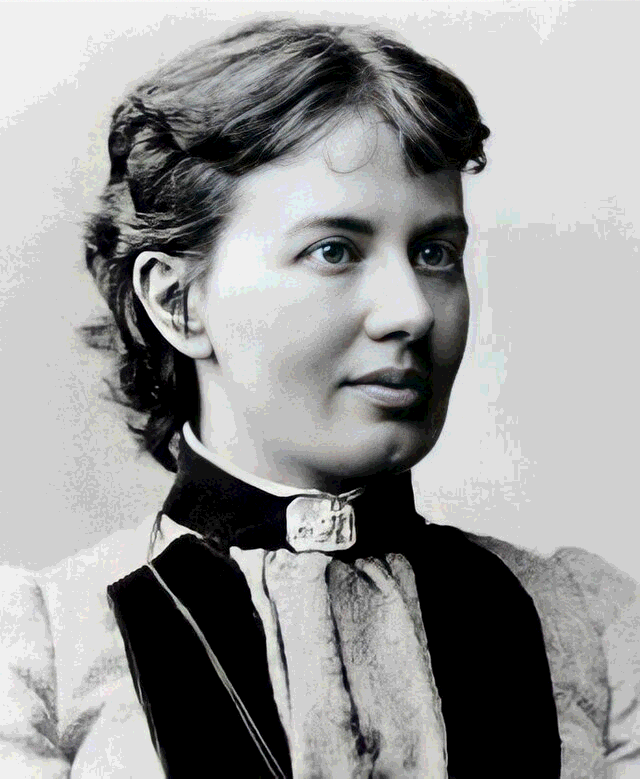
\includegraphics[width=\linewidth]{img/sofya-4-5.png}
		\caption{4 бита.}
		\label{fig:p4}
	\end{subfigure}
	\hfill
	\begin{subfigure}[b]{0.3\linewidth}
		\centering
		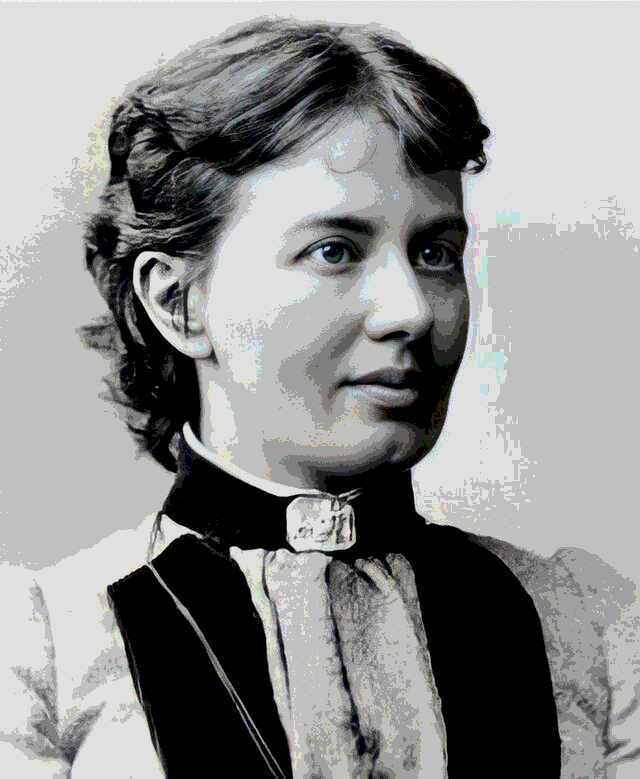
\includegraphics[width=\linewidth]{img/sofya-5-5.png}
		\caption{5 бит.}
		\label{fig:david5}
	\end{subfigure}
	\hfill
	\begin{subfigure}[b]{0.3\linewidth}
		\centering
		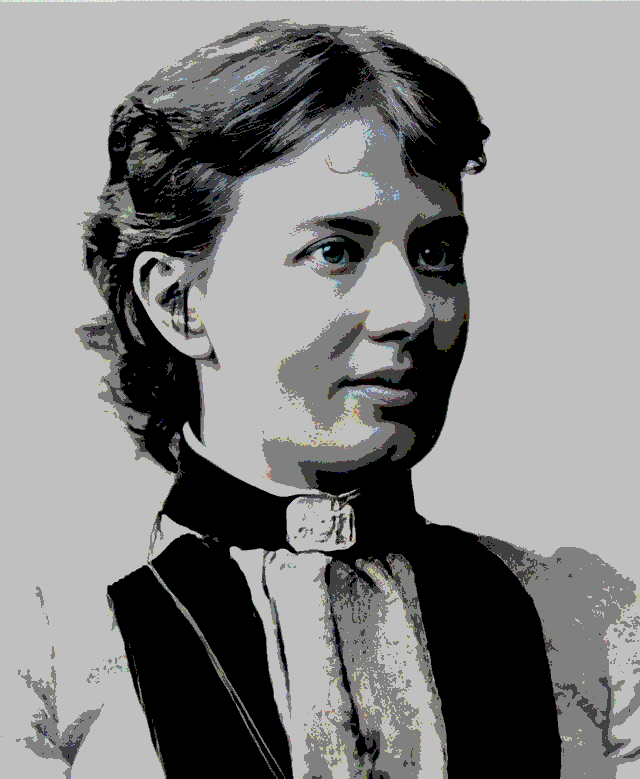
\includegraphics[width=\linewidth]{img/sofya-6-5.png}
		\caption{6 бит.}
		\label{fig:p6}
	\end{subfigure}
	
	\vspace{0.5cm}
	
	\begin{subfigure}[b]{0.3\linewidth}
		\centering
		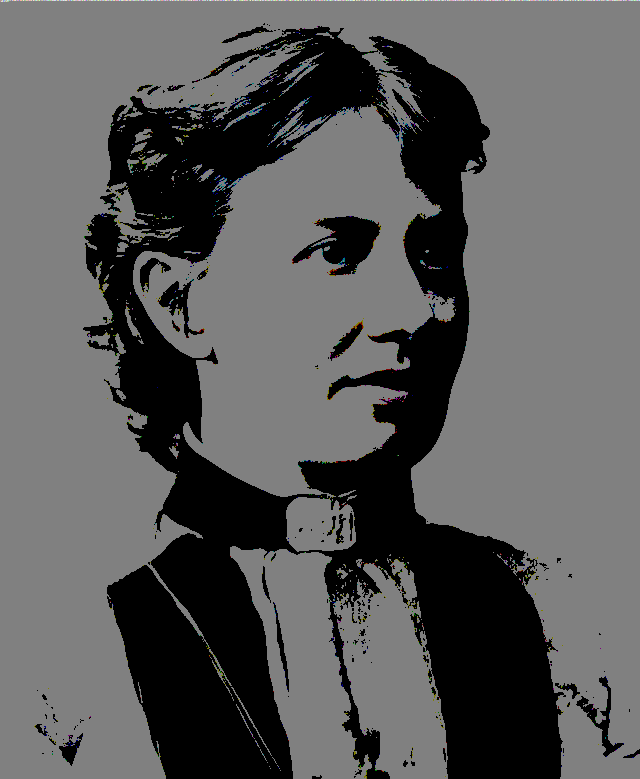
\includegraphics[width=\linewidth]{img/sofya-7-5.png}
		\caption{7 бит.}
		\label{fig:p7}
	\end{subfigure}
	\hspace{0.05\linewidth} % Для выравнивания влево
	\begin{subfigure}[b]{0.3\linewidth}
		\centering
		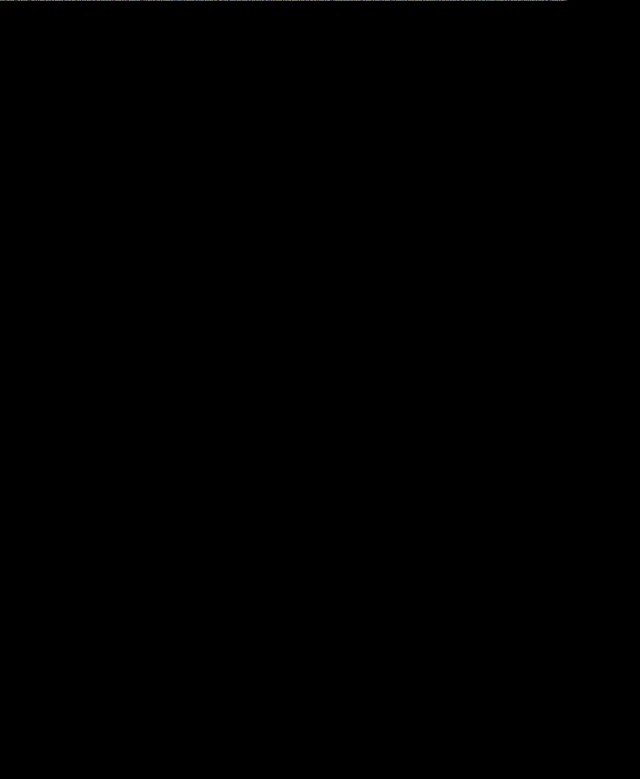
\includegraphics[width=\linewidth]{img/sofya-8-5.png}
		\caption{8 бит.}
		\label{fig:p8}
	\end{subfigure}
	
	\caption{Изображения с зашифрованными данными.}
	\label{fig:encrypted_images_rest}
\end{figure}

\newpage
На \hyperref[fig:encrypted_images_row1]{рисунках 3а--3c} и \hyperref[fig:encrypted_images_rest]{4а--4е} представлены результирующие изображения с разным количеством бит, отведённых под зашифрованные данные.

\subsection{Второй вариант}
Аналогично первому случаю, программа при успешном завершении создаст три файла с выводом в консоль путей сохранения файлов и изображения. Результаты работы программмы в консоли представлены на \hyperref[fig:res2]{рис. 5.}

\newpage
\begin{figure}[h]
	\centering
	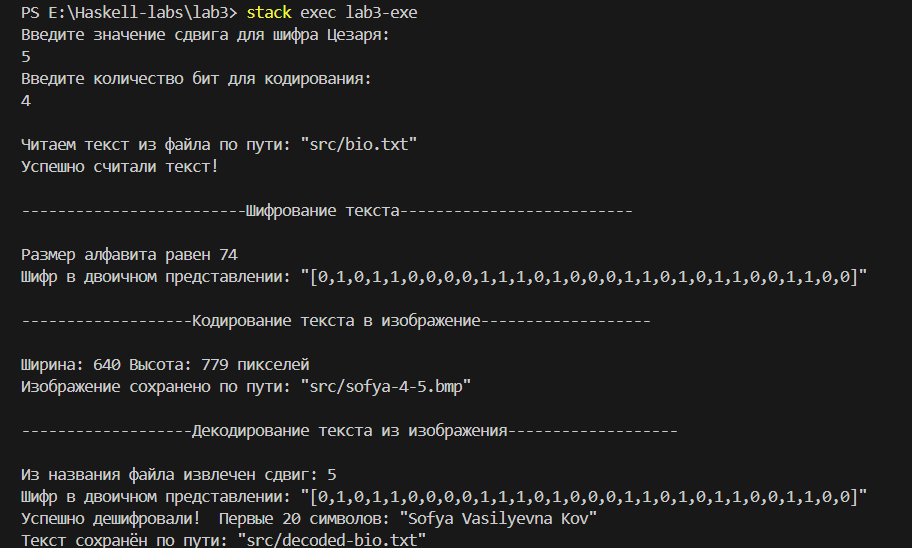
\includegraphics[width=0.75\linewidth]{img/res2.png}
	\caption{Результаты работы программы в консоли.}
	\label{fig:res2}
\end{figure}


% Первая строка на первой странице
\begin{figure}[h!]
	\centering
	\begin{subfigure}[b]{0.3\linewidth}
		\centering
		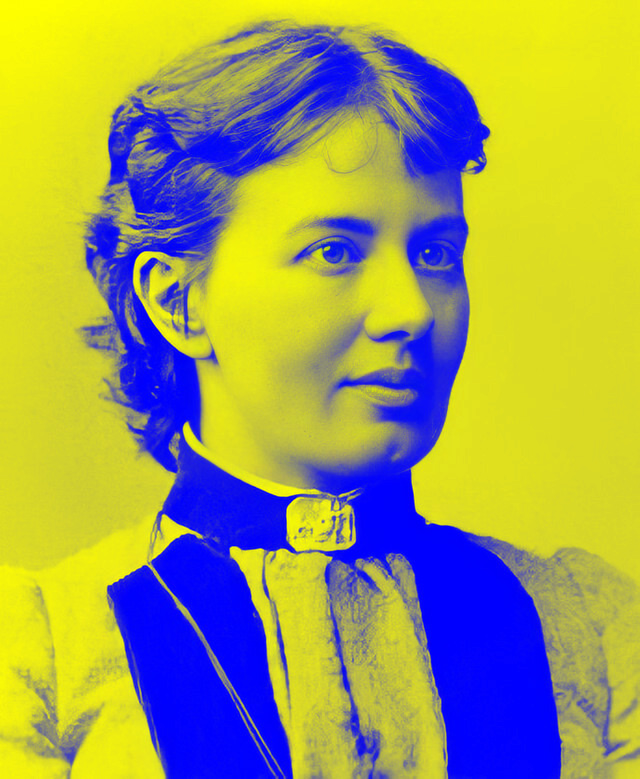
\includegraphics[width=\linewidth]{img/sofya2-1-5.jpg}
		\caption{1 бит.}
		\label{fig:s1}
	\end{subfigure}
	\hfill
	\begin{subfigure}[b]{0.3\linewidth}
		\centering
		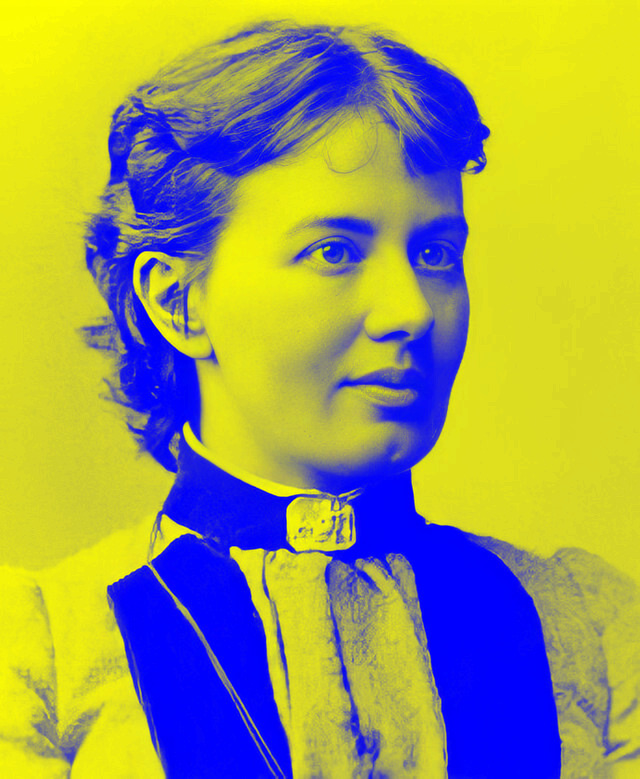
\includegraphics[width=\linewidth]{img/sofya2-2-5.jpg}
		\caption{2 бита.}
		\label{fig:s2}
	\end{subfigure}
	\hfill
	\begin{subfigure}[b]{0.3\linewidth}
		\centering
		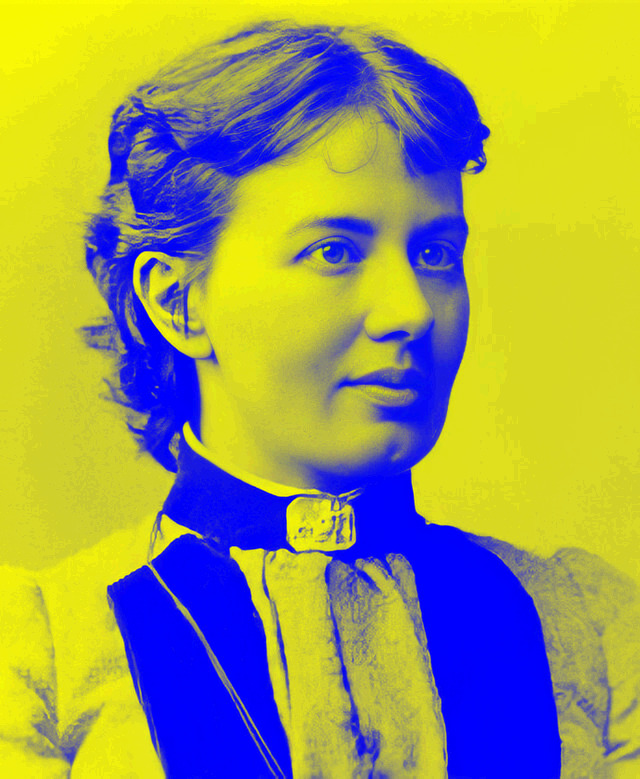
\includegraphics[width=\linewidth]{img/sofya2-3-5.jpg}
		\caption{3 бита.}
		\label{fig:s3}
	\end{subfigure}
	
	\begin{subfigure}[b]{0.3\linewidth}
		\centering
		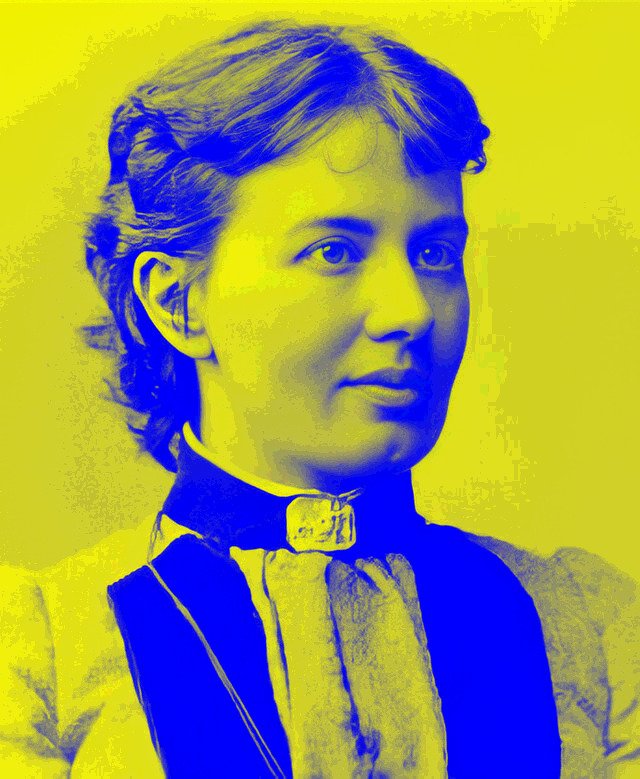
\includegraphics[width=\linewidth]{img/sofya2-4-5.jpg}
		\caption{4 бита.}
		\label{fig:s4}
	\end{subfigure}
	\hfill
	\begin{subfigure}[b]{0.3\linewidth}
		\centering
		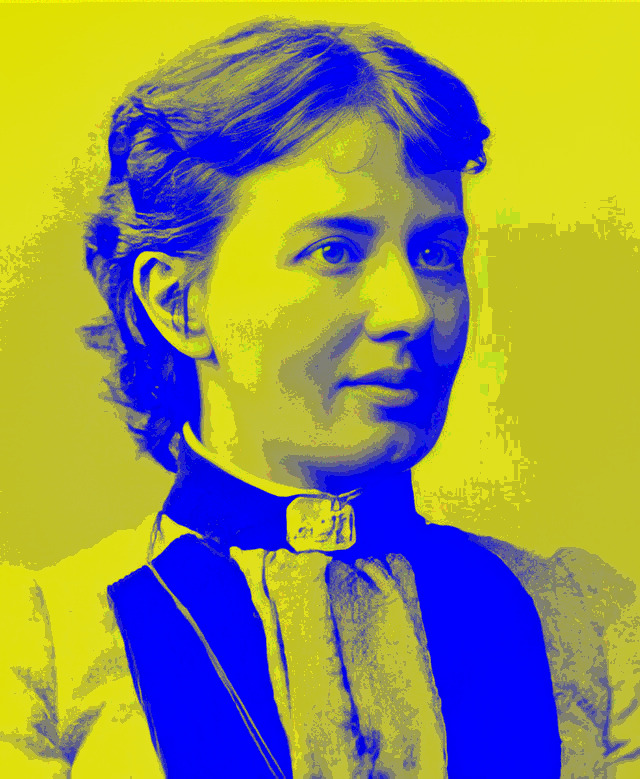
\includegraphics[width=\linewidth]{img/sofya2-5-5.jpg}
		\caption{5 бит.}
		\label{fig:s5}
	\end{subfigure}
	\hfill
	\begin{subfigure}[b]{0.3\linewidth}
		\centering
		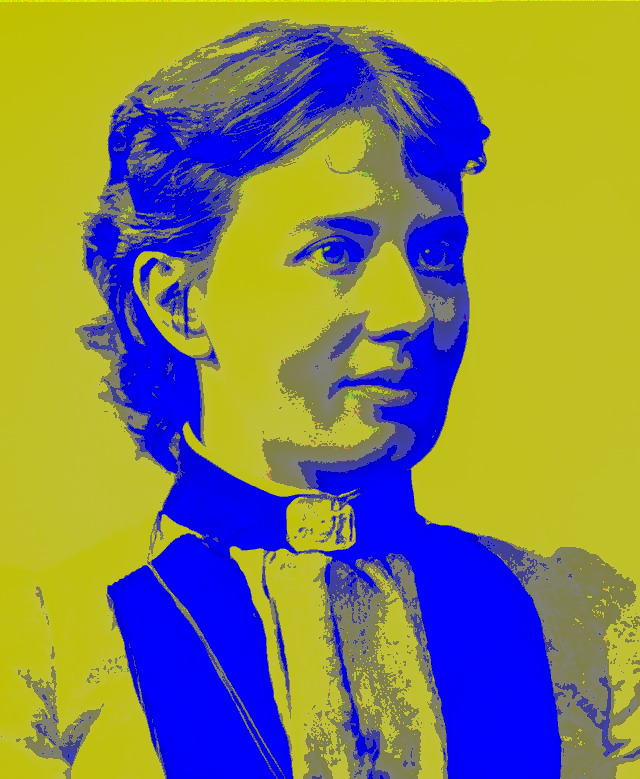
\includegraphics[width=\linewidth]{img/sofya2-6-5.jpg}
		\caption{6 бит.}
		\label{fig:s6}
	\end{subfigure}
	
	\caption{Изображения с зашифрованными данными.}
	\label{fig:new1}
\end{figure}

% Вторая часть: нумерация с d
\begin{figure}[h!]
	\centering
	
	\begin{subfigure}[b]{0.3\linewidth}
		\centering
		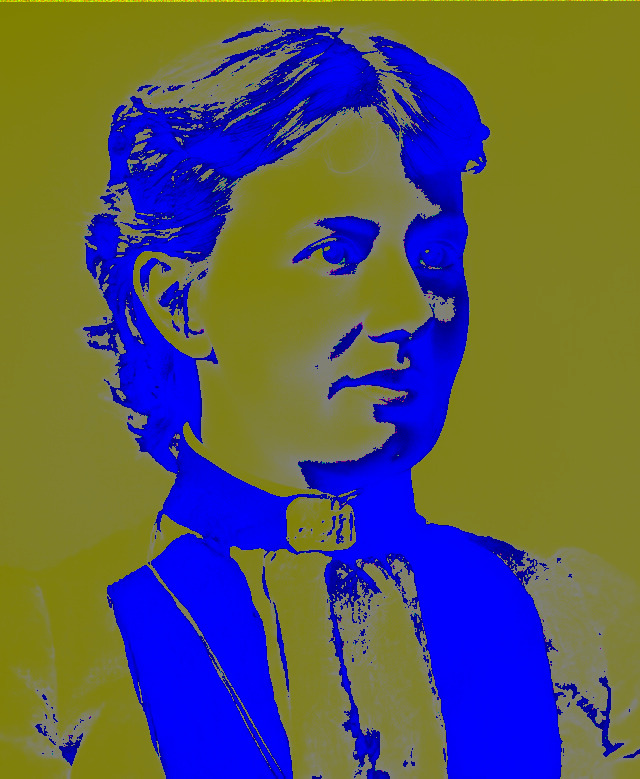
\includegraphics[width=\linewidth]{img/sofya2-7-5.jpg}
		\caption{7 бит.}
		\label{fig:s7}
	\end{subfigure}
	\hspace{0.05\linewidth} % Для выравнивания влево
	\begin{subfigure}[b]{0.3\linewidth}
		\centering
		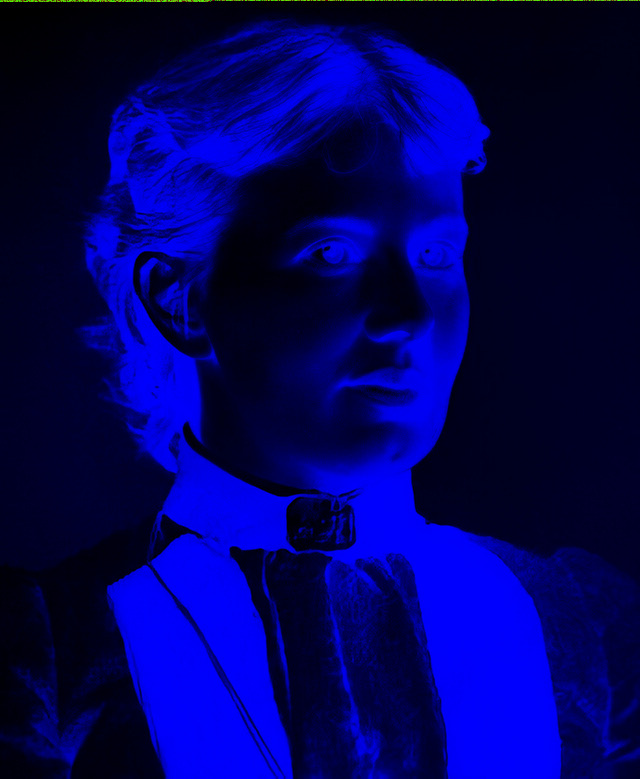
\includegraphics[width=\linewidth]{img/sofya2-8-5.jpg}
		\caption{8 бит.}
		\label{fig:s8}
	\end{subfigure}
	
	\caption{Изображения с зашифрованными данными.}
	\label{fig:new2}
\end{figure}












На \hyperref[fig:new1]{рисунках 6а--6f} и \hyperref[fig:new2]{7а--7b} представлены результирующие изображения с разным количеством бит, отведённых под зашифрованные данные.








\newpage
\section*{Заключение}
\addcontentsline{toc}{section}{Заключение}
В результате выполнения лабораторной работы была создана программа на языке Haskell, которая способна кодировать текстовые данных из указанного файла с помощью шифра Цезаря и сохранять эти данные внутрь изображения. Причём программа позволяет выбрать как смещение для шифра Цезаря, так и количество бит, которое будет использовано в каждом байте изображения для хранения данных. 


\newpage
\addcontentsline{toc}{section}{Список литературы} % Добавляем раздел в содержание

\vspace{-1.5cm}
\begin{thebibliography}{0}
	\bibitem{caesar}
	Luciano, D., Prichett, G., Cryptology: From Caesar Ciphers to Public-Key Cryptosystems, The College Mathematics Journal, 1987.
	\bibitem{david}
	David Deutsch -- personal website, URL: \url{https://www.daviddeutsch.org.uk/}, Дата обращения: 19.11.2024
	\bibitem{convertio}
	Convertio -- BPM to JPG online converter, URL: \url{https://convertio.co/ru/bmp-jpg/}, Дата обращения: 19.11.2024
	\bibitem{JuicyPixels}
	Hackage -- JuicyPixels: Picture loading/serialization, URL: \url{https://hackage.haskell.org/package/JuicyPixels}, Дата обращения: 19.11.2024
\end{thebibliography}



	
\end{document}